\documentclass[10pt,a4paper]{article}
\usepackage[centertags]{amsmath}
\usepackage{amsfonts,amssymb, amsthm}
\usepackage{hyperref}
\usepackage{comment}
\usepackage[shortlabels]{enumitem}
\usepackage{bm}

\usepackage{cite,graphicx,color}
%\usepackage{fourier}
\usepackage[margin=1.5in]{geometry}
\usepackage{enumitem}
\usepackage{bbm}

\usepackage{tikz,pgfplots}

\usepackage{mathtools}
%\mathtoolsset{showonlyrefs} % only show no. of refered eqs

\usepackage{cleveref}

\textheight 8.5in

\newtheorem{theorem}{Theorem}
\newtheorem{assumption}{Assumption}
\newtheorem{example}{Example}
\newtheorem{proposition}{Proposition}

\newtheoremstyle{dotlessP}{}{}{\color{blue!50!black}}{}{\color{blue}\bfseries}{}{ }{}
\theoremstyle{dotlessP}
\newtheorem{question}{Question}



\def\VV{\mathbb{V}}
\def\EE{\mathbb{E}}
\def\PP{\mathbb{P}}
\def\RR{\mathbb{R}}
\newcommand{\mD}{\mathcal{D}}
\newcommand{\mF}{F}%{\mathcal{F}}

\DeclareMathOperator{\sgn}{sgn}
%\DeclareMathOperator{\erf}{erf}
\DeclareMathOperator{\erfc}{erfc}
\DeclareRobustCommand{\argmin}{\operatorname*{argmin}}
\DeclareRobustCommand{\arginf}{\operatorname*{arginf}}

\def\EE{\mathbb{E}}\def\PP{\mathbb{P}}
\def\NN{\mathbb{N}}\def\RR{\mathbb{R}}\def\ZZ{\mathbb{Z}}



\def\<{\left\langle} \def\>{\right\rangle}


%\DeclareRobustCommand{\linear}{\operatorname*{Linear}}
%\DeclareRobustCommand{\loss}{\operatorname*{Loss}}
%\DeclareRobustCommand{\diag}{\operatorname*{diag}}

\newcommand{\linear}{\text{Linear}}
\newcommand{\loss}{\text{Loss}}
\newcommand{\diag}{\text{diag}}




\newcommand{\emphasis}[1]{\textcolor{red!80!black}{#1}}
\newcommand{\shanyin}[1]{\textcolor{blue!80!black}{#1}}

% ****************************
\begin{document}


\title{Deep learning HW2}
\author{Shanyin Tong, st3255@nyu.edu}

\maketitle


\section{Theory}

\subsection{Convolutional Neural Netoworks}
\begin{enumerate}[(a)]
	\item The number of kernels for height $n_H$ satisfies: $2(n_H-1)+3\leq 10$, so $n_H=4$. The number of kernels for width $n_W$: $2(n_W-1)+3\leq 11$, so $n_W=5$. The output is the total kernels: $n_H\times n_W=4\times5$.
	
	The output dimension is $4\times5$.
	\item The input channel is $C$, since apply $F$ filters, the output will have $F$ matrices. For a single image/matrix in input, it is size $H\times W$. Use padding $P$, the size becomes $(H+2P)\times(W+2P)$. The kernel size is $K\times K$, with dilation $D$, it becomes $[(K-1)D+1]\times[(K-1)D+1]$. As in (a), assume $n_H$ and $n_W$ are the number of kernels can be applied to the height and width. With stride $S$, we have
	\begin{equation*}
	\begin{aligned}
	(n_h-1)S+(K-1)D+1\leq H+2P &\Rightarrow && n_h = 1+\left\lfloor\frac{H+2P-[(K-1)D+1]}{S}\right\rfloor\\
	(n_w-1)S+(K-1)D+1\leq W+2P&\Rightarrow&& n_w = 1+\left\lfloor\frac{W+2P-[(K-1)D+1]}{S}\right\rfloor,
	\end{aligned}
	\end{equation*}
	where $\lfloor\cdot\rfloor$ is rounding a number down to the nearest integer.
	
	So the output dimension is $F\times\left( 1+\left\lfloor\frac{H+2P-[(K-1)D+1]}{S}\right\rfloor\right) \times \left(1+\left\lfloor\frac{W+2P-[(K-1)D+1]}{S}\right\rfloor \right) $.
	
	\item \begin{enumerate}[(i)] 
		\item Since filter is 1, there is 1 output channel. For input dimension 5, kernel size 3 and stride 2 with no padding or dilation, the output dimension $n_W$ satisfies $2(n_W-1)+3\leq 5$, thus $n_W=2$. 
		
		So the output $f_W(x)\in\RR^{1\times 2}$. The element of $f_W(x)$ is 
		\begin{equation}
		f_W(x)[i,j] = \sum_{k=1}^{3} W[i,:,k] x[2j-2+k]=\sum_{k=1}^{3} \sum_{l=1}^2W[i,l,k] x[l,2j-2+k],\;i=1,\; j=1,2.
		\end{equation}
		Here, I consider $x[n]$ as column vector and $W[i,:,k]$ is a row vector.
		
		
		\item Here, I use the same notations for matrix gradients as in the book "Mathematics for Machine Learning", and same for the following answers.
		
		Since $W\in\RR^{1\times 2\times 3}$ and $f_W(x)\in\RR^{1\times 2}$,
		\begin{equation}
		\frac{\partial f_W(x)}{\partial W}\in \RR^{(1\times 2)\times (1\times 2\times 3)},
		\end{equation}
		its element is 
		\begin{equation}
		\begin{aligned}
		\frac{\partial f_W(x)}{\partial W}[i,j,k,l,m]=\frac{f_W(x)[i,j]}{\partial W[k,l,m]}
=  x[l,2j-2+m],\\
		 i=1,\; j=1,2,\; k=1,\; l=1,2,\;m=1,2,3.
		\end{aligned}
		\end{equation}
		
		\item Since $f_W(x)\in\RR^{1\times 2}$ and $x\in\RR^{2\times 5}$, 
		\begin{equation}
		\frac{\partial f_W(x)}{\partial x}\in\RR^{(1\times 2) \times (2\times 5) },
		\end{equation}
		its element is 
		\begin{equation*}
		\begin{aligned}
		\frac{\partial f_W(x)}{\partial x}[i,j,k,l]=\frac{\partial f_W(x)[i,j]}{\partial x[k,l]}=\left\lbrace 
		\begin{aligned}
	&	W[i,k,l+2-2j], & \text{ if } l+2-2j\in\{1,2,3\},\\
	&	0, & \text{ else,}
		\end{aligned}
		\right. \\i=1,\; j=1,2, \; k=1,2, \; l=1,\ldots, 5.
		\end{aligned}
		\end{equation*}
		
		\item Different from what we uses in homework 1 (numerator-layout). To keep the homework 2 consistent, I use the denominator-layout notation$\frac{\partial l}{\partial f_W(x)}\in \RR^{1\times 2}$ and $\frac{\partial l}{\partial f_W(x)}[i,j]=\frac{\partial l}{\partial f_W(x)[i,j]}$ Thus, 
		\begin{equation}
		\frac{\partial l}{\partial W}\in \RR^{1\times 2 \times 3},
		\end{equation}
		its element is 
		\begin{equation}
		\begin{aligned}
		\frac{\partial l}{\partial W}[i,j,k]=&\frac{\partial l}{\partial W[i,j,k]}
		= \sum_{q=1}^2\frac{\partial l}{\partial f_W(x)[1,q]}\frac{\partial f_W(x)[1,q]}{\partial W[i,j,k]}\\
		=&\sum_{q=1}^2\frac{\partial l}{\partial f_W(x)[1,q]} x[j,2q-2+k]\\
		= &\frac{\partial l}{\partial f_W(x)[1,1]} x[j,k]+\frac{\partial l}{\partial f_W(x)[1,2]} x[j,2+k], \\
		&i=1,\; j=1,2,\; k=1,2,3.
		\end{aligned}
		\end{equation}
		
		The expression in (i) is the forward pass for convolutional neural network, while in (iv) the formula is its backward pass. The similarity for both pass is they all have locality/sparsity, i.e., they all require some of the input data $x[n]$, but not the full $x$ for one neuron computation. The difference is for forward pass, it requires three neighboring input samples $x[n]$ to compute one output $f_W(x)[:,j]$, while the downward pass require input sample $x[n]$ with the corresponding stride, i.e. $x[1]$ and $x[3]$ for $\frac{\partial l}{\partial W}[i,j,1]$, $x[2]$ and $x[4]$ for $\frac{\partial l}{\partial W}[i,j,2]$, $x[3]$ and $x[5]$ for $\frac{\partial l}{\partial W}[i,j,3]$. The other similarity is stationarity, i.e. the pass share the some parameter for different neurons. The output for forward pass $f_W[i,1]$ and $f_W[i,2]$ share the same weight $W$, while the gradient for downward pass $\frac{\partial l}{\partial W}[i,j,1], \frac{\partial l}{\partial W}[i,j,2], \frac{\partial l}{\partial W}[i,j,3]$ share the gradient $\frac{\partial l}{\partial f_W(x)}$ and $x$.
	\end{enumerate}
\end{enumerate}
\newpage
\subsection{Recurrent Neural Networks}
\begin{enumerate}[(a)]
	\item  The diagram for this recurrent neural network is 
	\begin{figure}[tbhp]\centering
		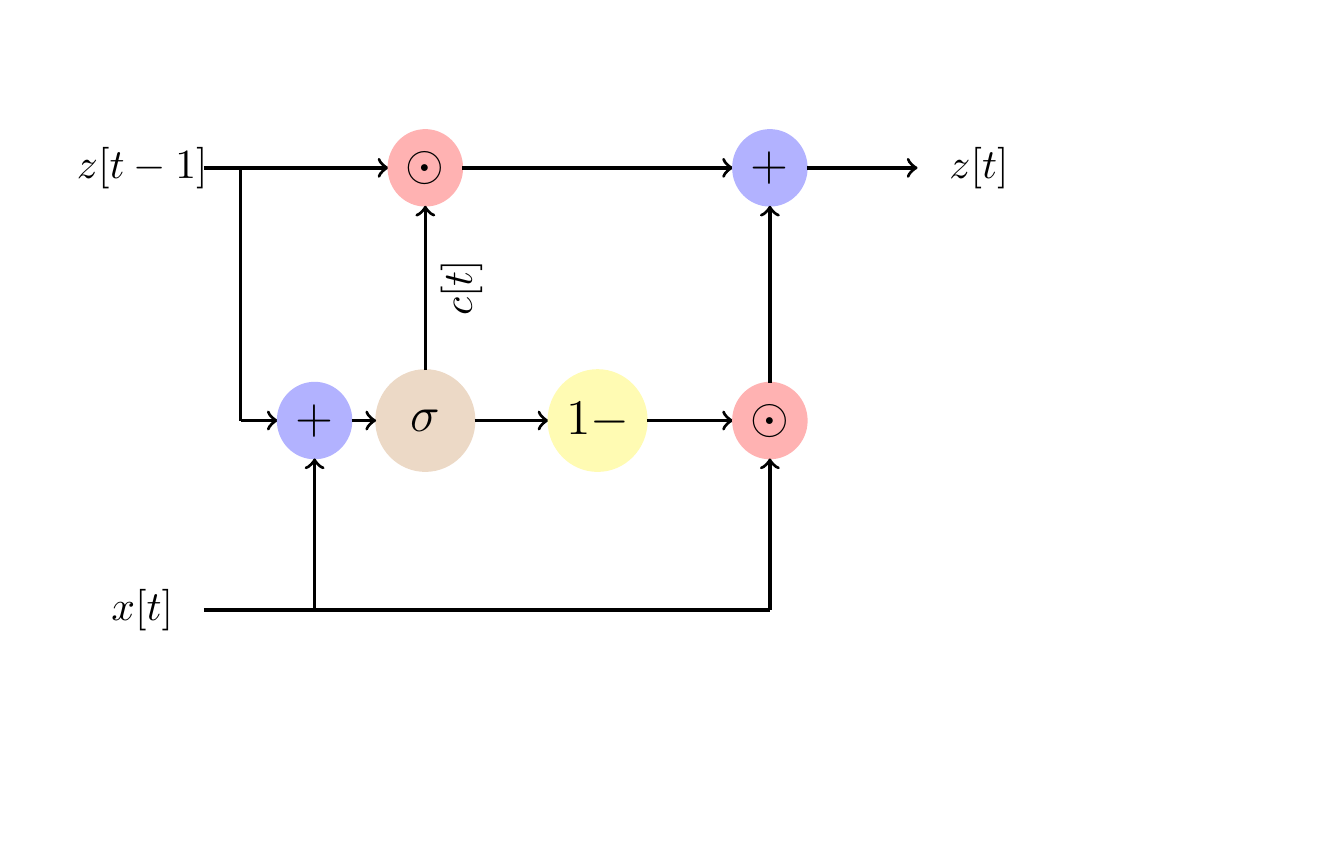
\begin{tikzpicture}[scale = 1.5]
		\begin{axis}[compat=1.11, width=12cm, height=8cm,
		xmin=-5,
		xmax=5,
		ymin=-3,
		ymax=3,
		axis line style={draw=none},
		tick style={draw=none},
		yticklabels={,,},
		xticklabels={,,},
		]
		\node at (-4.3,2) {$z[t-1]$};
		\draw[->, thick](-3.8,2) -- (-2.3,2);
		\filldraw [red!30] (-2,2) circle (.3) node[black]{\large $\odot$};		
		\draw[thick](-3.5,2) -- (-3.5,0);
		\draw[thick,->](-3.5,0) --(-3.2,0);
		\filldraw [blue!30] (-2.9,0) circle (.3) node[black]{\large $+$};
		\filldraw [brown!30] (-2,0) circle (.4) node[black]{\large $\sigma$};
		\draw[thick,->](-2.6,0) --(-2.4,0);	
		\draw[thick,->] (-2,0.4) -- (-2,1.7) node[midway,sloped, below]{$c[t]$};
		\draw[thick,->](-1.6,0) --(-1,0);		
		\filldraw [yellow!30] (-0.6,0) circle (.4) node[black]{\large $1-$};		
			\draw[thick,->](-0.2,0) --(0.5,0);		
			\filldraw [red!30] (0.8,0) circle (.3) node[black]{\large $\odot$};		
			\draw[->, thick](-1.7,2) -- (0.5,2);
			\filldraw [blue!30] (0.8,2) circle (.3) node[black]{\large $+$};
		\draw[->,thick] (-2.9, -1.5) -- (-2.9,-0.3);
		\node at (-4.3,-1.5) {$x[t]$};
		\draw[thick](-3.8,-1.5) -- (0.8,-1.5);
		\draw[->,thick] (0.8, -1.5) -- (0.8, -0.3);
		\draw[->,thick] (0.8, 0.3) -- (0.8, 1.7);
		\draw[->,thick] (1.1, 2) -- (2, 2);
		\node at (2.5,2) {$z[t]$};
		\end{axis}
		\end{tikzpicture}
	\end{figure}
	\item Since $c(t)$ and $z(t)$ are in the same size, the dimension of $c(t)$ is $c(t)\in \RR^m$.
	
	\item Use the denominator-layout notation, since $W_x \in \RR^{m\times n}$, thus $\frac{\partial l}{\partial W_x}\in \RR^{m\times n}$, its element is
	\begin{equation}\label{eq:dldW}
	\begin{aligned}
	\frac{\partial l}{\partial W_x}[i,j] =&\frac{\partial l}{\partial W_x[i,j]}\\
 =&\sum_{t=1}^{K} \sum_{p=1}^m \frac{\partial l}{\partial z[t][p]}\frac{\partial z[t][p]}{\partial W_x[i,j]}\\
 =& \sum_{t=1}^{K}  \frac{\partial l}{\partial z[t][i]} \frac{\partial z[t][i]}{\partial W_x[i,j]}\\
 =&\frac{\partial l}{\partial z[1][i]}(1-c[1][i])x[1][j]+\sum_{t=2}^{K}  \frac{\partial l}{\partial z[t][i]} \left[ c[t][i]\frac{\partial z[t-1][i]}{\partial W_x[i,j]} + (1-c[t][i])x[t][j]\right] \\
 =&  \sum_{t=1}^{K} \frac{\partial l}{\partial z[t][i]}  \sum_{s=1}^{t}  x[s][j](1-c[s][i])
 \prod_{r\leq t, r>s} c[r][i], \\
 & i=1,\dots, m, \; j=1,\ldots, n.
	\end{aligned}
	\end{equation}
	Note when $s\geq t$, we use $ \prod_{r\leq t, r>s} c[r][i]=1$.
	
	The forward pass and backward pass in this RNN all use $c[t]$ to control if use the information from the input $x[t]$ at time $t$. If $c[t][i]=1$, then in the forward pass, the output $z[t][i]$ do not use input data $x[t]$ but use the memory $z[t-1]$. While in the downward pass, $\frac{\partial l}{\partial W_x}[i,:]$ is zero, meaning it also do not use the input info $x[t]$. When $c[t][i]=0$, it means in the forward pass we use the previous data $x[s], s\leq t$ to compute the output $z[t]$, so we may accumulate $x[s]$ in our output, so the corresponding gradient from the downward pass will also accumulate the influence.
	
	\item This RNN can help prevent vanishing or exploding gradients. Assume $x[t]$ and $\frac{\partial l}{\partial z[t]}$ are nonzero element-wisely.  According to \eqref{eq:dldW}, the gradient 
	\begin{equation}
	\frac{\partial l}{\partial W_x}[i,j]=\sum_{t=1}^{K} \frac{\partial l}{\partial z[t][i]}  \sum_{s=1}^{t}  x[s][j] A(i,t,s) 
	,
	\end{equation}
	 the coefficient $A(i,t,s)$ is
	\begin{equation}\label{eq:coef}
A(i,t, s):=	(1-c[s][i])
	\prod_{r\leq t, r>s} c[r][i] \in \{0, 1\}, \; s\leq t,
	\end{equation}
	
	If $c[p][i]=0$, then $A(i,t,s)=0, s<p\leq t$; if $c[p][i]=1$, then $A(i,t,p)=0$, so either case for $c[p][i]$, there are several coefficient $A(i,t,s)$'s are zeros, so this prevent the exploding for gradient.
	
	Let $k=\text{argmax}\{r: c[r][i] = 0\}$, if $k$ exists, then $A(i,t ,k)$ is nonzero for $t\geq k$. If $k$ does not exit, this means we do not use any input $x[t]$, which is a rare case. For the other cases, we always have some $A(i,t ,k)$'s are nonzero. This prevents vanishing gradients.
\end{enumerate}
\end{document}